% Chapter Template

\chapter{GNSS Systems Overview} % Main chapter title

\label{Chapter2} % Change X to a consecutive number; for referencing this chapter elsewhere, use \ref{ChapterX}

The format of this chapter is as follows, there is a section on the details behind GNSS systems and the history behind GNSS and how it came to be in its current state. After that
an overview of the current and future GNSS constellations including operating principles was covered. Then real world uses of GNSS are listed. Following that the errors
that account for the inaccuracies of calculated GNSS position are covered, including the definition of spoofing types.

%----------------------------------------------------------------------------------------
%	SECTION 1
%----------------------------------------------------------------------------------------

\section{History of GNSS Systems} \label{sec:GNSSHistory}
In 2021 there are many different GNSS systems in place that service the globe. It is a technology that has become deeply ingrained in the everyday lives of most
people around the world. The first digital based navigation system similar to what we know today was the use of terrestrial based radio transmitters in the form of
hyperbolic navigation systems \cite{RN68}. The concept was
similar to that of the current satellite based systems, namely the use of pseudoranges, although the accuracy was far lower than is acceptable today. The USA developed
and commissioned the first satellite based navigation system.

As of 2021 there are six operational GNSS systems in use. These are GPS (USA), GLONASS (Russia), Galileo (EU), BeiDou (China), IRNSS/NavIC (India) and QZSS (Japan). The
QZSS system currently acts to complement the coverage of GPS in the East Asian and Oceanic regions with 4 operational satellites. There are plans to increase this number
of satellites to allow for stand alone use as a GNSS provider \cite{RN47}. The Indian IRNSS similarly provides regional coverage around India with 8 satellites in
geostationary orbit \cite{RN55} . There are three categories of orbit, LEO, MEO and GEO. These are categorised by how far from the earths surface the satellite orbits.
Current GNSS systems utilise MEO orbits.

GNSS, and more specifically GPS and GLONASS, date back to 1957 during the space race between the USA and the then USSR \cite{RN43}. When Russian satellite Sputnik 1 was
launched scientists at the John Hopkins University were able to track its position and velocity by measuring the Doppler shift of the craft. This tracking from Doppler
shift measurements continued with the launch of the subsequent satellites Sputnik 2 and Explorer 1. After this it was thought that the process could be reversed such that
a satellite with a known position could be used to resolve an unknown position on earth. In the 1960's the TRANSIT satellite navigation system was made operational for US
Navy use, mainly for position and navigation of nuclear ballistic missile submarines. TRANSIT received strong support due to the accuracy of up to 80ft (24m) which was a
significant improvement over existing VLF (Very Low Frequency) hyperbolic navigation systems. After 32 years of operation the system was retired in 1996 after proving
that space crafts could be reliable \cite{RN45}. 

In 1973 the US combined two existing programs in TIMATION and 'Project 621B' to form the 'NAVSTAR Global Positioning System' which would later become known more
commonly as GPS. The initial intention for the use of GPS was for military only. However, in 1983 there was an incident that saw a Korean Airlines flight shot down by a
Soviet fighter mistaking it for a US aircraft when it wandered off course. After this incident President Reagan announced that GPS would be made available for civilian
use. The military insisted that the accuracy of the system be purposely degraded for civilian use though selective availability such that GPS could not be used by
adversaries. In 1993 the system was declared operational. To combat the intentional accuracy reduction of the GPS augmentation systems started to appear. Soon
after there were Government funded versions of DGPS (Differential GPS) systems \cite{RN43}. Augmentation systems significantly increases the accuracy by using a receiver
with a known location and having that receiver calculate its position from the satellite signals and compare with the known position. These corrections are then
broadcast. 

The Soviet Union launched their first GLONASS satellite in 1982, and in the following three years 10 more were launched. There are some technical differences between the
GLONASS and GPS constellations. The orbital planes are different and GLONASS uses an FDMA (Frequency Division Multiple Access) scheme as opposed to the GPS CDMA (Code
Division Multiple Access). In 1993 president Yeltsin declared that the GLONASS constellation was fully operational, however this was not the case. 

The TRANSIT satellite system orbit was in a LEO (Low Earth Orbit) polar orbit, whereas all modern GNSS systems utilise a MEO (medium earth orbit) ranging from 20,000km to
23,000km above the earths surface with multiple orbital planes. The number of planes differs between the different constellations as discussed below. The lower the orbit,
the higher the velocity required to maintain the orbit as shown by the orbital mechanics equation \ref{eq:orbitalVelocity}. Equally a higher orbit requires a lower
velocity which has impact on the Doppler shift at the receivers. Another factor is aerodynamic drag, which is higher the closer to the earths surface due to the
atmosphere.

\begin{equation} \label{eq:orbitalVelocity}
    v \approx \frac{2\pi a}{T} \approx \sqrt{\frac{\mu_{earth}}{a}}
\end{equation} 

The history of the two other main GNSS systems is much shorter, with the Galileo constellation coming as a form of sovereignty for the European Union. The fist satellite
was launched in 2011, and the service became operational in 2016. There is also a network of GPS augmentation sites that provide improved accuracy for those in the EU.
This system is named EGNOS. This system provided an average of 1.5m accuracy over the EU territory. This was provided through the use of ground stations and a
geostationary satellite broadcasting the timing corrections. 

%----------------------------------------------------------------------------------------
%	SECTION 2
%----------------------------------------------------------------------------------------

\section{GNSS Systems} \label{sec:GNSS}
\subsection{Introduction to GNSS Constellations}\label{subsec:GNSS_Intro}
GNSS is a term used to describe any satellite system that provides position and timing information. All GNSS systems in use today have three separate segments that
encompass the term GNSS. That is the ground segment, space segment and user segment. These are used in conjunction to allow the user to calculate with accuracy up to $\pm
10cm$. In order to calculate an unknown position on Earth, the exact position of the orbiting satellite must be known. The satellite will send it's exact position as well
as it's current time down to Earth's surface. It's location, or ephemeris, can be tracked due to Kepler's laws and celestial mechanics. The time on board satellites is
kept via the use of caesium based atomic clocks. The GPS clocks are accurate to approximately 10 nanoseconds \todo{reference}, however, receivers will lose timing due to
the interpretation of signals and typically provide accuracy of 100 nanoseconds. The value of the clocks are constantly monitored by the ground segment and updated when
required. Part of the receivers (the user segment) will pick up this signal. The components of the message sent are quite simple and consist mostly of the current time
(of the satellite) and where the satellite is in the WGS-84 coordinate system\cite{RN46}. This coordinate system has its origin at the centre of mass of the earth with
the Z axis pointing at the north pole, the X axis pointing towards the prime meridian and the y axis perpendicular to both other axes. Due to the relative motion of the
satellite and the receiver the transmitted signal will be shifted up or down the frequency range due to the Doppler effect. The combination of this Doppler shift, time
taken to arrive and the satellite current location can be used to solve the position in three dimensional space. In order to solve for all dimensions (including time)
four satellites are required since there are essentially 4 unknown terms to solve for as shown in equation \ref{eq:gnssPosition} \cite{RN46}. The $\rho_i$ term indicates
the distance from the receiver at the time of reception to that particular satellite at time of transmission  and is known as a pseudorange. $x_i$, $y_i$ and $z_i$ are
the coordinates of the $i_{th}$ satellite in three dimensional space as dictated by the ECEF (Earth Centered Earth Fixed) coordinate system. This coordinate system is a
version of a Cartesian coordinate systems where the origin is at the center of mass of the earth. $x_u$, $y_u$ and $z_u$ are the unknown coordinates of the receiver. The
coordinates of all satellites are well known due to the distribution of the ephemeris. By getting 3 satellites, the unknown values can be solved using simultaneous
equation techniques. The $\Delta t$ is the error in the clock of the sender and receiver. Any drift in time will be multiplied by the speed of light and can cause very
large errors with only a small drift in time. Therefore to get a proper three dimensional fix with high accuracy, a minimum of 4 satellites are required.  

This method of position calculation is known as trilateration. The model shown below is a simplified model that ignores the effects of relativity. 

\begin{equation} \label{eq:gnssPosition} 
    \rho_i = \sqrt{(x_i - x_u)^2 + (y_i - y_u)^2 + (z_i - z_u)^2} + c \Delta t
\end{equation}
As can be seen from the above equation \ref{eq:gnssPosition} the accurate synchronisation of time between the receiver and the satellites is required in order to
calculate an accurate position. 
Each of the operational constellations use the same fundamentals to provide accurate position data, but each differ in some key aspects as discussed below.

\subsection{Trilateration} \label{subsec:Trilateration}
The process of trilateration uses objects of known locations to calculate the unknown location of other objects. This is done through the use of overlapping circles based
on how far the objects are apart. This is known as a pseudorange. To use satellites to determine the location of a receiver the exact location of the satellites must be
known, as well as relative distance. Each satellite sends its precise orbital location (ephemeris), as well as the coarse orbital location (almanac) of the rest of the
constellation as part of the navigational data. This coupled with the pseudorange of the satellite allows for calculating the position of the receiver. Pseudoranges rely
on the knowledge that electromagnetic radiation propagates at the speed of light, as shown in equation \ref{eq:EMdistance}. By measuring the time taken for the signal to
transition from the each of the satellites to the receiver, a sphere of radius $d$ centred on the radius indicates all possible locations that the receiver could be. By
adding a second satellite, and second sphere based on the pseudorange, the possible locations of the receiver are reduced based on where the spheres intersect. For 2D
position only 3 satellites are needed to have only a single possible solution, whereas 3 dimensional position requires 4 satellites as shown in Figure
\ref{fig:trilateration}.

\begin{equation} \label{eq:EMdistance}
    d = c \times t
\end{equation}

\begin{figure}[h]
    \begin{centering}
        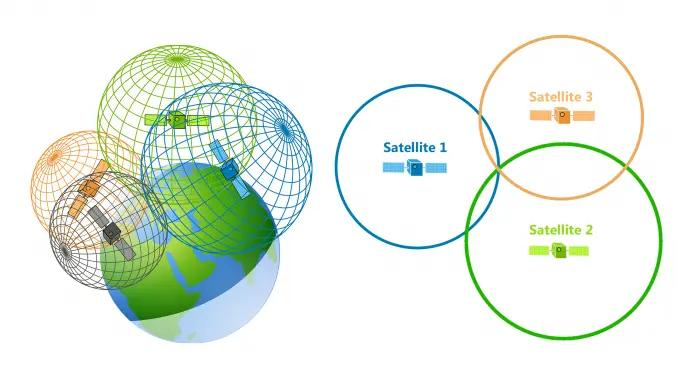
\includegraphics[width=14cm,keepaspectratio]{Figures/trilateration.png}
        \caption{Illustration of trilateration used in GNSS positioning}
        \label{fig:trilateration}
    \end{centering}
\end{figure}

\subsection{Kepler's Laws of Planetary Motion} \label{subsec: OrbitalMechanics}
In the 1600's German astronomer Johannes Kepler described the orbits of the solar systems planets around the sun using three laws. 
These laws famously moved our understanding of orbits away from circles and described them as ellipses. The position of modern day satellites need to be accurately
predicated and as such these laws have become important to the way we live our lives. Kepler's laws are as follows; First law states that the orbit of every planet is an
ellipse with the sun at the one of the two foci. Second law states that a line joining the planet to the sun will sweep out equal area during equal intervals of time.
The third law states that the ratio of the orbital period with the cube of the semi-major axis is the same for all objects orbiting the same primary. These laws can be
adapted to objects that orbit other objects other than the sun. Examples are moons orbiting planets and artificial satellites orbiting the earth.

\subsection{GPS} \label{subsec:GNSS_GPSIntro}
The GPS constellation consists of a nominal 24 satellites in 6 orbital planes (nominally 4 satellites per plane) to ensure that there is coverage globally at all times.
There are also some spare satellites that are in orbit in the event that a operational satellite malfunctions. The constellation orbits at an altitude of 20,200km which
equates to an orbital period of 12hours. There are multiple frequencies of differing properties that each satellite will transmit at. For GPS these are named the L1, L2
and L5 bands and have centre frequencies of 1575.42MHz, 1227.60MHz and 1176.45MHz respectively \cite{RN49}. This is shown graphically in Figure \ref{fig:SignalPlan}. The
L1 band is the most commonly used and was the first one to be made operational. In the past the L1 band was used for civilian purposes and the L2 band was a military
band. Nowadays both have active civilian and encrypted signals co-exiting within their respective frequency bands. GPS predominately uses BPSK (Binary Phase Shift Keying)
but also utilises  (Binary Offset Keying) for signal modulation across all of the bands. 

All satellites within the constellation will broadcast using the same frequency band (L1, L2 or L5). They are able to do this without interfering through the use of CDMA
(Code Division Multiple Access) scheme. Each satellite has a unique chipping code that is used to spread the signal in the frequency domain. This code is a PRN (Pseudo
Random Number). This same access scheme is used for GPS, Galileo and BeiDou.

Initially the civilian C/A code was purposely degraded to ensure that adversaries of the USA could not use the system to its maximum effect. In May 2000 President Bill
Clinton directed the removal of selective availability from the GPS service, and in 2007 it was announced that the newest version of GPS satellites would be manufactured
without the selective availability capability \cite{RN62} \cite{RN64}.

GPS hardware has had a number of revisions over the life of the system in the form of Blocks. Each block is a major revision, current generation satellites are Block III
satellites. Block I satellites were only capable of transmitting on the L1 and L2 bands and only had a 5 year design life. Block II maintained the same transmitting
frequency capabilities as before but included three axis stabilisation provided by reaction wheels. The solar arrays were increased from a rated 410W to over 700W. Later
iterations of Block II included the L2C band for more robust civil signals and improvement to the military signal.
There are currently 4 block III satellites in service with 6 more planned for launch. There are 12 block IIF satellites in operation which were launched from
2010 to 2016. Block IIR has 8 currently operational from 13 launches, block IIR-M has 7 operational from 8 launches and there are no operational satellites from Block I,
II or IIA. This totals 31 operational satellites, 24 in operation and 7 spares as summarised in Table \ref{tab:GPSSatSum}

Accuracy of the GPS system has increased over the years, and since selective availability was legislated against, to approximately 3m for public access and 3-4cm for
encrypted.

% \renewcommand{\arraystretch}{1.5}
% \begin{table}
%     \begin{center}
%         \caption{Summary of current and former GPS satellites}
%         \label{tab:GPSSatSum}
%         \begin{tabular}{ |r|c|c| }
%             \hline
%             \textbf{Block} & \textbf{Launched} & \textbf{In Service} \\
%             \hline
%             Block I & 11 & 0\\
%             \hline
%             Block II & 9 & 0\\
%             \hline
%             Block IIA & 19 & 0\\
%             \hline
%             Block IIR & 13 & 8\\
%             \hline
%             Block IIR-M & 8 & 7\\
%             \hline
%             Block IIF & 12 & 12\\
%             \hline
%             Block III & 4 & 4\\
%             \hline
%             \hline
%             \textbf{Total} & \textbf{76} & \textbf{31}\\
%             \hline
%         \end{tabular}
%     \end{center}
% \end{table}
% \renewcommand{\arraystretch}{1}

\renewcommand{\arraystretch}{1.5}
\begin{table}
    \begin{center}
        \caption{Summary of current and former GPS satellites}
        \label{tab:GPSSatSum}
        \begin{tabular}{ r|c|c }
            \hline
            \textbf{Block} & \textbf{Launched} & \textbf{In Service} \\
            \hline
            Block I & 11 & 0\\
            Block II & 9 & 0\\
            Block IIA & 19 & 0\\
            Block IIR & 13 & 8\\
            Block IIR-M & 8 & 7\\
            Block IIF & 12 & 12\\
            Block III & 4 & 4\\
            \hline
            \textbf{Total} & \textbf{76} & \textbf{31}\\
            \hline
        \end{tabular}
    \end{center}
\end{table}
\renewcommand{\arraystretch}{1}

\subsection{Galileo} \label{subsec:GNSS_GalileoIntro}
The Galileo constellation is a GNSS created by the ESA (European Space Agency) and operated by the EGA (European GNSS Agency) as a way of providing a modern navigation
system that has global coverage. The Galileo constellation has 30 nominal satellites across 3 orbital planes. The first Galileo satellite was launched in 2011.
The orbit height of the Galileo constellation is higher than the GPS orbit at 23,222 km. 

Galileo operates on 3 different frequency bands, E1, E5 and E6. E1 shares the same centre frequency as the GPS L1 band, 1575.42 MHz. The E6 band does not share a frequency
with the GPS system and operates at 1278.75 MHz. The E5 band is split into E5a and E5b sub-bands with E5a sharing the same frequency as L5, 1176.45 MHz, and E5b at
1207.14 MHz. The arrangement of the frequency bands can be seen in Figure \ref{fig:SignalPlan} \cite{RN69}.

\begin{figure}[h]
    \begin{centering}
        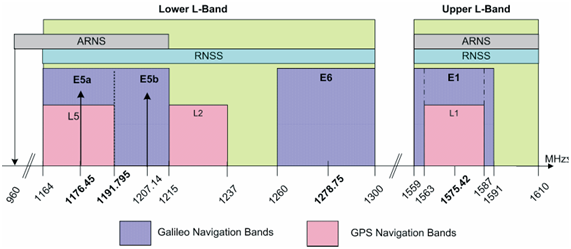
\includegraphics[width=14cm,height=10cm,keepaspectratio]{Figures/Galileo_Frequency_Plan.png}
        \caption{Galileo and GPS signal frequency arrangement \cite{RN69}}
        \label{fig:SignalPlan}
    \end{centering}
\end{figure}

To maintain interoperability between receivers on the L1 and E1 bands the modulation schemes differ.
The E1 band utilises Composite BOC modulation, E6 utilises BPSK, and the E5 bands utilise Alternative BOC modulation.
Galileo offers superior accuracy than the other constellations with 1m for the public access and 1cm for encrypted service.

There are special satellites that are part of the Galileo constellation whose job it is to ensure validity. These are known as GIOVE (Galileo In Orbit Validation Element)
satellites. There is GIOVE-A and GIOVE-B launched in 2005 and 2008 respectively. Initially these satellites transmitted GNSS test signals on the E1 and E6 frequency
bands to allow for monitoring and testing while the rest of the Galileo constellation was being commissioned \cite{RN65}. Over this time they have provided great information on the
short and long term reliability and accuracy of the on board atomic clocks \cite{RN66}.

\subsection{GLONASS} \label{subsec:GNSS_GLONASSIntro}
The Russian GLONASS constellation has it's history tightly intertwined with that of GPS and the space race, as mentioned above in \ref{sec:GNSSHistory}.
GLONASS consists of a nominal 24 satellites in 3 orbital planes. Since GLONASS uses FDMA, each satellite needs to transmit on a unique frequency \cite{RN56}. This is in contrast to
all other GNSS systems that use CDMA. Extra effort must therefore be applied to the reception of the signals since Doppler effects must be carefully considered. 
The use of FDMA does make GLONASS more resilient against jamming and spoofing attacks. In a CDMA system, like GPS, all satellites share the same carrier frequency
(ignoring the Doppler Effect), thus if an attack is performed all satellites are susceptible. Where as the GLONASS satellites all occupy separate frequency bands making a
system wide attack much harder and more expensive to perform. This was the motivation of using FDMA over CDMA initially. The use of FDMA over CDMA also causes and
interoperability issue when considering multi constellation support. The receiver must become much more complex in order to support not only multiple carrier frequencies
of different constellations but also due to the different access schemes. This increases cost and complexity where Galileo is much more compatible for this use case.
There are
three frequency bands that GLONASS operates in, L1, L2 and L3. These are separate to the L1, L2 of GPS \cite{RN70}. 

GLONASS L1 band is from 1598.0625 MHz to 1605.375 MHz split into 14 channels. Each carrier is 562.5 kHz apart and is characterised by equation \ref{eq:GLONASS Channel
calc}. $k$ represents the channel number of the band and ranges from -7 to +6. 

The L2 band ranges from 1242.9375 MHz to 1248.625 MHz with each carrier separated by 437.5 kHz.

The L3 band ranges from 1197.9375 MHz to 1203.625 MHz with the same carrier separation as L2.

\begin{equation} 
    \begin{split} \label{eq:GLONASS Channel calc}
        f_{k_{L1}} = f_{0_{L1}} + k \Delta f_{L1} \\ 
        f_{k_{L2}} = f_{0_{L2}} + k \Delta f_{L2} \\ 
        f_{k_{L3}} = f_{0_{L3}} + k \Delta f_{L3}
    \end{split}
\end{equation}

\subsection{BeiDou} \label{subsec:GNSS_BeiDouIntro}
From the BeiDou official website it states that "BeiDou has been constructed and operated by China with an eye on the needs of the country's national security, economic
and social development", and was previously known as COMPASS. This is China's attempt at creating a sovereign navigation constellation.

The BeiDou constellation is made up of 35 satellites in total. This includes 5 geostationary satellites, 27 MEO satellites and 3 inclined geosynchronous satellites to
give total earth coverage. The MEO satellites orbit at a height of 21,500km, and are distributed across 3 orbital planes. Through the use of the geostationary and
geosynchronous satellites there is a region around Asia that has higher accuracy than what is present at other areas of the globe. This accuracy for open service is
approximately 2.6m around the Asia Pacific region and 3.6m elsewhere \cite{RN59}. The constellation contains 3 operating bands, B1, B2 and B3, which have frequencies as shown in Table
\ref{tab:Beidou Signal}. Each of the bands use the CDMA access scheme.

% \renewcommand{\arraystretch}{1.5}
% \begin{table}
%     \begin{center}
%         \caption{Summary of BeiDou Signal Properties \cite{RN59}}
%         \label{tab:Beidou Signal}
%         \begin{tabular}{ |r|c|c| }
%             \hline
%             \textbf{Signal} & \textbf{Carrier Frequency (MHz)} & \textbf{Modulation Type} \\
%             \hline
%             B1-I & 1561.098 & BPSK\\
%             \hline
%             B1-Q & 1561.098 & BPSK\\
%             \hline
%             B1-C & 1575.420 & MBOC(6,1,1/11)\\
%             \hline
%             B1 & 1575.420 & BOC(14,2)\\
%             \hline 
%             \hline
%             B2-I & 1207.140 & BPSK\\
%             \hline
%             B2-Q & 1207.140 & BPSK\\
%             \hline
%             B2a & 1176.460 & AltBOC(15,10)\\
%             \hline
%             B2b & 1207.140 & AltBOC(15,10)\\
%             \hline 
%             \hline
%             B3-I & 1268.520 & BPSK\\
%             \hline
%             B3-Q & 1268.520 & BPSK\\
%             \hline
%             B3-A & 1268.520 & BOC(15,2.5)\\
%             \hline
%             B3 & 1268.520 & BPSK\\
%             \hline
%         \end{tabular}
%     \end{center}
% \end{table}
% \renewcommand{\arraystretch}{1}

\renewcommand{\arraystretch}{1.5}
\begin{table}
    \begin{center}
        \caption{Summary of BeiDou Signal Properties \cite{RN59}}
        \label{tab:Beidou Signal}
        \begin{tabular}{ r|c|c }
            \hline
            \textbf{Signal} & \textbf{Carrier Frequency (MHz)} & \textbf{Modulation Type} \\
            \hline
            B1-I & 1561.098 & BPSK\\
            B1-Q & 1561.098 & BPSK\\
            B1-C & 1575.420 & MBOC(6,1,1/11)\\
            B1 & 1575.420 & BOC(14,2)\\
            \hline
            B2-I & 1207.140 & BPSK\\
            B2-Q & 1207.140 & BPSK\\
            B2a & 1176.460 & AltBOC(15,10)\\
            B2b & 1207.140 & AltBOC(15,10)\\
            \hline
            B3-I & 1268.520 & BPSK\\
            B3-Q & 1268.520 & BPSK\\
            B3-A & 1268.520 & BOC(15,2.5)\\
            B3 & 1268.520 & BPSK\\
            \hline
        \end{tabular}
    \end{center}
\end{table}
\renewcommand{\arraystretch}{1}

\subsection{Augmentation Systems} \label{subsec:GNSS_OtherIntro}
As mentioned above there are two other GNSS constellations that act to improve availability and accuracy in regional areas. These are the Japanese QZSS and Indian
IRNSS. Both of these extend the abilities of the USA GPS system. The 4 satellites that are operational for the QZSS constellation are able to transmit on the L1 and L5
band  simultaneously. Doing so helps to resolve ionospheric errors by facilitating resolution of position from multiple frequencies \cite{RN48}.

The IRNSS constellation is different to the others mentioned above due to its orbit altitude of 36,000km making them geostationary. All of the satellites are positioned at
this orbit. This allows for a very narrow and defined region of usability, which is over India \cite{RN55}. 

Other forms of augmentation as mentioned in Section \ref{sec:GNSSHistory} were through ground based stations that use receivers to determine the timing error and broadcast these
values in order to make the solution to the position calculation more accurate. This type of system allows for sub 1m accuracy. These systems are typically rolled out
geographically locally and run by those local Governments.

\subsection{GNSS Receivers}
Traditional GNSS receivers are specialised hardware components that are able to receive the spread spectrum signal from the GNSS satellite and perform the required
calculations to acquire the PVT data. This data is then provided serially to a main processor of the system in the form of NMEA (National Marine Electronics Association)
sentences, see \ref{subsubsec:NMEA}. There are many sentence types
and not all receivers will output all sentence types.

\subsubsection{NMEA Sentences} \label{subsubsec:NMEA}
The NMEA (National Maritime Electronics Association) has a number of standards one of which is NMEA-0183. This standard outlines the combined electrical and data
specifications for communication between marine electronic equipment. The data specification was adopted by GPS receiver manufacturers to ensure software could operate
with any GPS hardware. The standard outlines the typical message structure. This structure lays the foundation for many different message types called sentences. These
sentences carry different information depending on the sentence type, and it is often the case that multiple sentences will be required in order for the software to
understand the full picture. One of the key inclusions within the data specification is the checksum. Each sentence has a checksum based on the contents of the message
that can be easily checked to ensure no data was corrupted in the transmission process. The checksum method is XOR based where each character between the delimiting
characters are XOR'd together and their integer value is used as the checksum.

Each of the main constellations has their own unique "Talker Identifier Mnemonics" as dictated by the NMEA-0183 standard Table 7 \todo{insert citation}, which is summarised
below in Table \ref{tab:NMEA Mnemonics}. This allows for easy differentiation of PVT sources without needing to know anything about the hardware itself.

% \renewcommand{\arraystretch}{1.5}
% \begin{table}
%     \begin{center}
%         \caption{GNSS Identifier Mnemonics as per NMEA-0183}
%         \label{tab:NMEA Mnemonics}
%         \begin{tabular}{ |l|c| }
%             \hline
%             \textbf{Talker Device} & \textbf{Identifier} \\
%             \hline
%             Galileo Positioning System & GA \\
%             \hline
%             BDS (BeiDou System) & GB \\
%             \hline
%             NavIC (IRNSS) & GI \\
%             \hline
%             Glonass Receiver & GL \\
%             \hline
%             Global Navigation Satellite System & GN \\
%             \hline
%             Global Positioning System (GPS) & GP \\
%             \hline
%             QZSS & GQ \\
%             \hline
%         \end{tabular}
%     \end{center}
% \end{table}
% \renewcommand{\arraystretch}{1}

\renewcommand{\arraystretch}{1.5}
\begin{table}
    \begin{center}
        \caption{GNSS Identifier Mnemonics as per NMEA-0183}
        \label{tab:NMEA Mnemonics}
        \begin{tabular}{ l|c }
            \hline
            \textbf{Talker Device} & \textbf{Identifier} \\
            \hline
            Galileo Positioning System & GA \\
            BDS (BeiDou System) & GB \\
            NavIC (IRNSS) & GI \\
            Glonass Receiver & GL \\
            Global Navigation Satellite System & GN \\
            Global Positioning System (GPS) & GP \\
            QZSS & GQ \\
            \hline
        \end{tabular}
    \end{center}
\end{table}
\renewcommand{\arraystretch}{1}

%----------------------------------------------------------------------------------------
%	SECTION 3
%----------------------------------------------------------------------------------------

\section{Applications of GNSS} \label{sec:ApplicationsGNSS}
GNSS applications are broad and deeply ingrained in almost everyone's everyday lives. These applications vary from providing position and navigation information for public
transport or maps on a smartphone or sat-nav devices to providing accurate timing information for financial institutions or energy infrastructure \cite{RN33} \cite{RN12}
as shown in Figure \ref{fig:GNSS Applications}. This societal ubiquity has made GNSS as much a critical infrastructure as internet or energy provision, since these
services rely on the services provided by GNSS.

\begin{figure}[h]
    \begin{centering}
        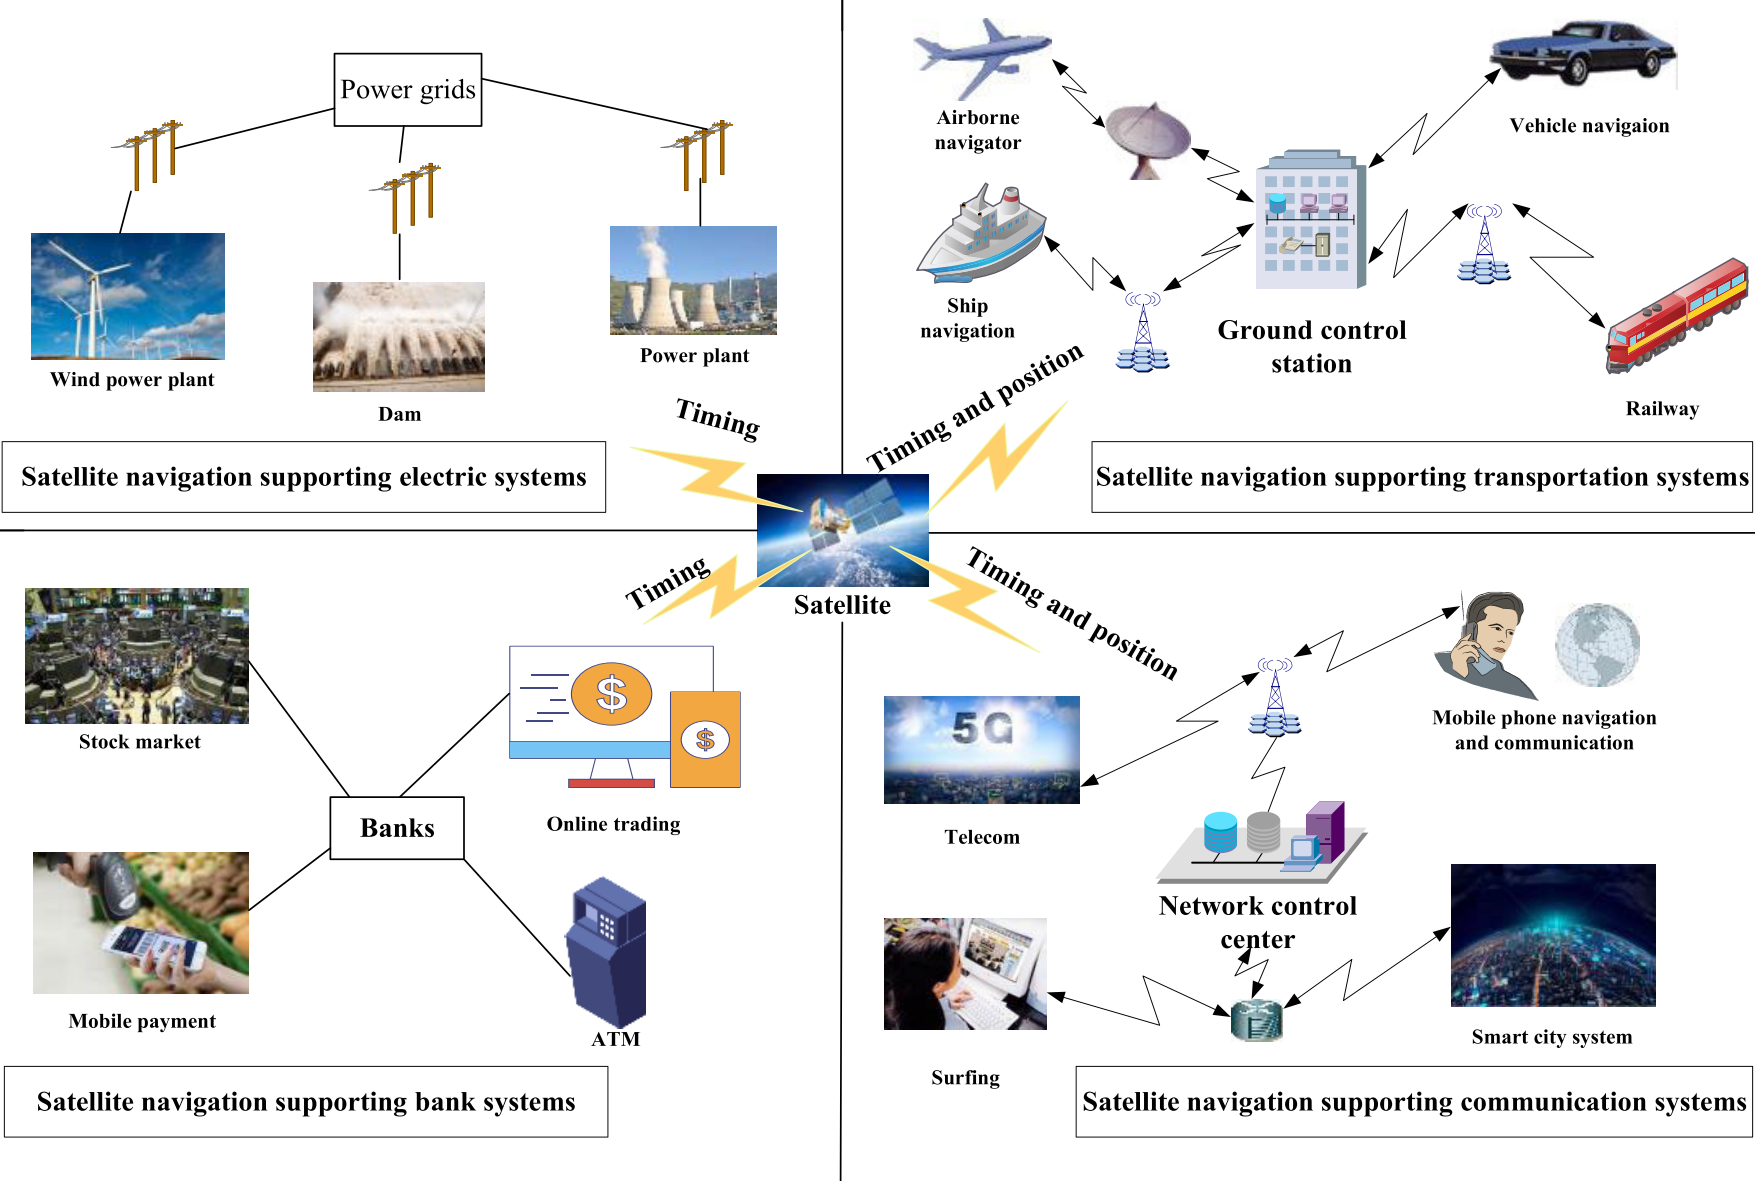
\includegraphics[width=14cm,keepaspectratio]{Figures/GNSS applications.png}
        \caption{Applications of GNSS position and timing \cite{RN33}}
        \label{fig:GNSS Applications}
    \end{centering}
\end{figure}

%----------------------------------------------------------------------------------------
%	SECTION 4
%----------------------------------------------------------------------------------------

\section{Errors within GNSS}
The main fight against GNSS positional accuracy is the introduction of different types of errors. These can be narrowed into three main groups; Satellite errors,
Propagation errors and Receiver errors. Propagation errors are most common. When the signals pass through the ionosphere and the troposphere the signals refract, extending
the time taken to get to the receiver, thus making the pseudorange not accurate. Other propagation errors include multipath and obstructions errors. Both of which are
most notable in built up urban environments of in valleys where direct view of the sky can be difficult.

Satellite errors occur when the predicated orbit differs to the actual orbit. Other causes of errors from the satellites are due to drift of the onboard atomic clocks as
well as low elevations where there are proportionally high dilution of precision.

Receiver errors occur due to the introduction of noise through the reception process. GNSS jamming and spoofing also constitute receiver error although these are
intentional and malicious.

What all of these errors have in common is that create an incorrect value of the pseudorange which in turn incorrectly calculates the receiver position.
\todo{ref}

\renewcommand{\arraystretch}{1.5}
\begin{table}
    \begin{center}
        \caption{Summary of GPS Errors}
        \label{tab:GPS Errors}
        \begin{tabular}{ c|c }
            \hline
            \textbf{Source of Error} & \textbf{Error Range} \\
            \hline
            Satellite Clocks & $\pm 2m$\\
            Orbital Errors & $\pm 2.5m$\\
            Ionospheric Delays & $\pm 5m$\\
            Tropospheric Delays & $\pm 0.5m$\\
            Receiver Noise & $\pm 0.3m$\\
            Multipath Errors & $\pm 1m$\\
            \hline
        \end{tabular}
    \end{center}
\end{table}
\renewcommand{\arraystretch}{1}

% \renewcommand{\arraystretch}{1.5}
% \begin{table}
%     \begin{center}
%         \caption{Summary of GPS Errors}
%         \label{tab:GPS Errors}
%         \begin{tabular}{ |c|c| }
%             \hline
%             \textbf{Source of Error} & \textbf{Error Range} \\
%             \hline
%             Satellite Clocks & $\pm 2m$\\
%             \hline
%             Orbital Errors & $\pm 2.5m$\\
%             \hline
%             Ionospheric Delays & $\pm 5m$\\
%             \hline
%             Tropospheric Delays & $\pm 0.5m$\\
%             \hline
%             Receiver Noise & $\pm 0.3m$\\
%             \hline
%             Multipath Errors & $\pm 1m$\\
%             \hline
%         \end{tabular}
%     \end{center}
% \end{table}
% \renewcommand{\arraystretch}{1}

%----------------------------------------------------------------------------------------
%	SECTION 5
%----------------------------------------------------------------------------------------

\section{Spoofing Overview}
Attacks on the GNSS architecture can broadly be divided into two categories jamming and spoofing \cite{RN33} \cite{RN32}. Jamming can be described as causing intentional
interference in the communication channel as to make the recovery of signal information impossible. A successful jamming attack will make it impossible to begin tracking
satellites and thus be unable to calculate any of the PVT data. This differs from spoofing attacks where the main interest is to deceive any receiver that picks ups the
signal into thinking it is elsewhere or else-when. This is done by different methods and stems from which property of the signal is being modified for the attack. A
successful spoofing attack will have the receiver 'tracking' the signal produced by the spoofer and the receiver will not be aware that an attack is taking place. Common
spoofing attacks are explained below.

\begin{figure}[h]
    \begin{centering}
        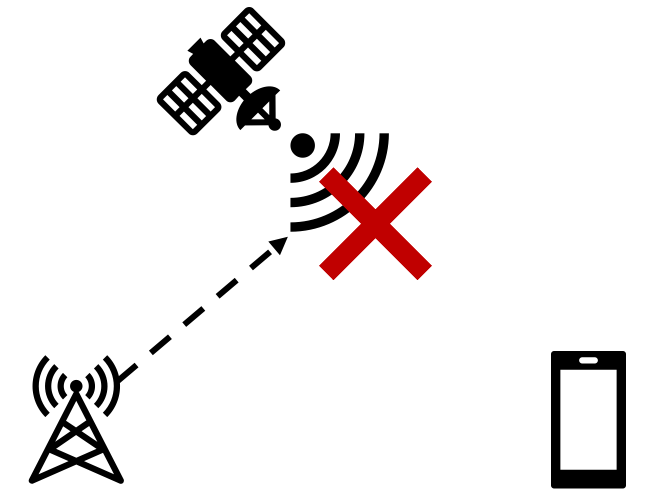
\includegraphics[width=10cm, keepaspectratio]{Figures/Jamming.png}
        \caption{Representation of how a jammer is able to interfere with a GNSS signal}
    \label{fig:jamming cartoon}
    \end{centering}
\end{figure}

\subsection{Meaconing}
Meaconing is a type of GNSS spoofing attack that involves recording a legitimate GNSS signal and re-broadcasting. This could be either instantly or at a different time or
place. This requires little prior knowledge of the GNSS system that the attacker wishes to record other when used with existing open source software packages. Although
there is a requirement of having the right equipment to be able to capture the raw analog signal.

\begin{figure}[h]
    \begin{centering}
        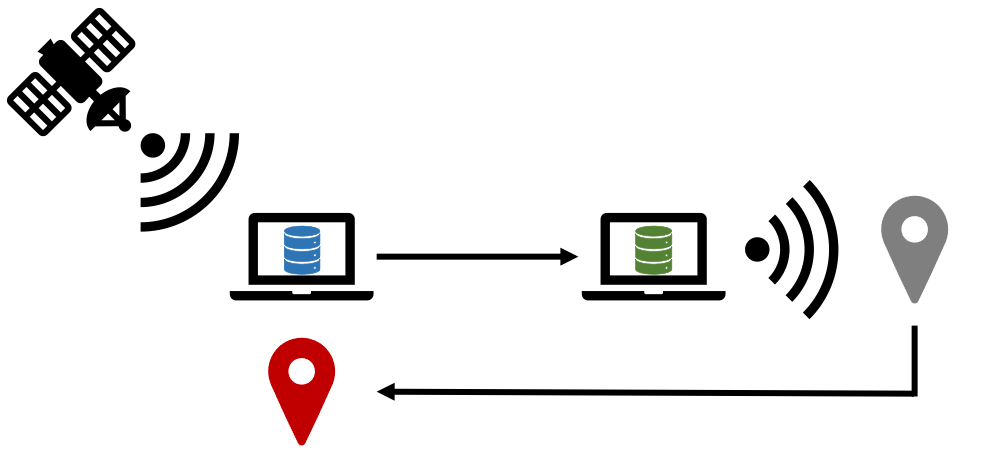
\includegraphics[width=12cm, keepaspectratio]{Figures/Meaconing.png}
        \caption{Representation of how a GNSS spoofer can perform a meaconing attack}
    \label{fig:meaconing cartoon}
    \end{centering}
\end{figure}

\subsection{Signal Generation}
There are software packages and off the shelf hardware that are designed for testing GNSS receivers in a laboratory setting. These can be used to generate a combination
of signals that can be
played in such a manner as to perform a spoofing attack. This differs from meaconing because knowledge of the satellite ephemeris and almanac is required. The almanac is
a record of the rough location of all satellites in a constellation and the ephemeris is the exact location of each individual satellite. This knowledge is required as to
produce the same results as recording the GPS signal from the desired location.

\begin{figure}[h]
    \begin{centering}
        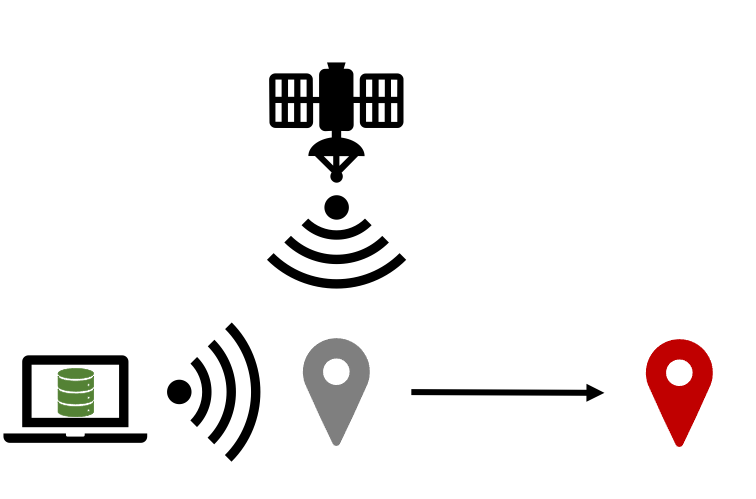
\includegraphics[width=10cm, keepaspectratio]{Figures/Spoofing.png}
        \caption{Representation of how a GNSS spoofing device uses a generated signal to force a receiver to incorrectly calculate its position}
    \label{fig:spoofing cartoon}
    \end{centering}
\end{figure}

%----------------------------------------------------------------------------------------
%	SECTION 6
%----------------------------------------------------------------------------------------

\section{SDR Basics} \label{sec:SDRBasics}
Software defined radios are devices that enable the user to increase the flexibility of transmission and reception of RF signals by moving processing typically reserved
for the analog domain into the digital domain. Thus SDRs move the signal processing from rigid and expensive hardware into flexible and in-expensive software. This
allows for a wide ranges of frequencies from Hz up to GHz from the same device with minor or no hardware changes. This can also be done in real time using software.
Typical tasks like modulation and demodulation are performed directly in analog hardware for normal radios. This makes them incredibly rigid and only suitable for 1 task.
An SDR can implement multiple different modulation/demodulation techniques and switch between them based on selection criteria set by the user. This same is true for
centre frequencies or carrier frequencies, they are able to be changed in real time from Hz to GHz depending on SDR model.

The USRP SDR lineup share the same basic block diagram design, as shown in Figure \ref{fig:USRPBlock}. This shows the way that the signals are transported from the analog
front end of the antenna through to the digital ethernet interface and vice-versa depending on whether transmitting or receiving. Also shown in figure \ref{fig:USRPBlock} is the
quadrature mixers which allow for complex sampling, shown in Equation \ref{eq:complexSampling} as apposed to real sampling, shown in Equation \ref{eq:realSampling}. This means that the in-phase and quadrature phase are sampled separately, effectively
doubling the sampling rate when compared to real only sampling. This means that when using complex sampling the Nyquist sampling theorem is conserved even when the
bandwidth is equal to the sampling rate.

SDRs need a device connected to them in order to off load processing of data and controlling radio parameters. This has typically been in the form of a PC or similar
device, but with recent technological advances SBCs (single board computer) and smartphones are powerful enough to handle this task. There are examples in literature of
using smartphones coupled with SDRs to perform many different radio based tasks.

\begin{equation} \label{eq:complexSampling}
    x\left(t\right) = A_{I}\left(t\right)\cos\left(2\pi f_{c}t\right) - A_{Q}\left(t\right)\sin\left(2\pi f_{c}t\right)
\end{equation}

\begin{equation} \label{eq:realSampling}
    x\left(t\right) = A\left(t\right)\cos\left(\omega t + \Phi \left(t\right)\right)
\end{equation}

\begin{figure}[h]
    \begin{centering}
        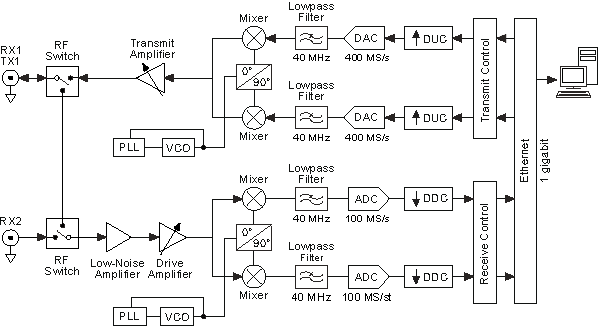
\includegraphics[width=13cm,keepaspectratio]{Figures/2920_simplified_system_diagram.png}
        \caption{Simplified block diagram for the RF front end of the USRP SDRs}
    \label{fig:USRPBlock}
    \end{centering}
\end{figure}